\documentclass[]{book}

%These tell TeX which packages to use.
\usepackage{array,epsfig}
\usepackage{amsmath}
\usepackage{amsfonts}
\usepackage{amssymb}
\usepackage{amsxtra}
\usepackage{amsthm}
\usepackage{mathrsfs}
\usepackage{color}
\usepackage{pgfplots}

%Here I define some theorem styles and shortcut commands for symbols I use often
\theoremstyle{definition}
\newtheorem{defn}{Definition}
\newtheorem{thm}{Theorem}
\newtheorem{cor}{Corollary}
\newtheorem*{rmk}{Remark}
\newtheorem{lem}{Lemma}
\newtheorem*{joke}{Joke}
\newtheorem{ex}{Example}
\newtheorem*{soln}{Solution}
\newtheorem{prop}{Proposition}

\newcommand{\lra}{\longrightarrow}
\newcommand{\ra}{\rightarrow}
\newcommand{\surj}{\twoheadrightarrow}
\newcommand{\graph}{\mathrm{graph}}
\newcommand{\bb}[1]{\mathbb{#1}}
\newcommand{\B}{\mathrm{B}}
\newcommand{\Z}{\bb{Z}}
\newcommand{\Q}{\bb{Q}}
\newcommand{\R}{\bb{R}}
\newcommand{\C}{\bb{C}}
\newcommand{\N}{\bb{N}}
\newcommand{\M}{\mathbf{M}}
\newcommand{\m}{\mathbf{m}}
\newcommand{\MM}{\mathscr{M}}
\newcommand{\HH}{\mathscr{H}}
\newcommand{\Om}{\Omega}
\newcommand{\Ho}{\in\HH(\Om)}
\newcommand{\bd}{\partial}
\newcommand{\del}{\partial}
\newcommand{\bardel}{\overline\partial}
\newcommand{\textdf}[1]{\textbf{\textsf{#1}}\index{#1}}
\newcommand{\img}{\mathrm{img}}
\newcommand{\ip}[2]{\left\langle{#1},{#2}\right\rangle}
\newcommand{\inter}[1]{\mathrm{int}{#1}}
\newcommand{\exter}[1]{\mathrm{ext}{#1}}
\newcommand{\cl}[1]{\mathrm{cl}{#1}}
\newcommand{\ds}{\displaystyle}
\newcommand{\vol}{\mathrm{vol}}
\newcommand{\cnt}{\mathrm{ct}}
\newcommand{\osc}{\mathrm{osc}}
\newcommand{\LL}{\mathbf{L}}
\newcommand{\UU}{\mathbf{U}}
\newcommand{\support}{\mathrm{support}}
\newcommand{\AND}{\;\wedge\;}
\newcommand{\OR}{\;\vee\;}
\newcommand{\Oset}{\varnothing}
\newcommand{\st}{\ni}
\newcommand{\wh}{\widehat}

%Pagination stuff.
\setlength{\topmargin}{-.3 in}
\setlength{\oddsidemargin}{0in}
\setlength{\evensidemargin}{0in}
\setlength{\textheight}{9.in}
\setlength{\textwidth}{6.5in}
\pagestyle{empty}



\begin{document}

\subsection*{Rappel de cours}

\begin{defn}
Soit $u \to ||u||$ une norme $\R^m$. La distance sur $\R^m$ est la fonction $d : \R^m \times \R^m \to  \R^+$ d\'efinie par $d(v,w) = ||w - v||$.
En particulier, on notera $d_1$; $d_{\infty}$; $d_2$ les distances associées à $|| . ||_1$; $k . k1$; $k . k2$. Donc :
\begin{itemize}
\item $d_1((x_1, \ldots. x_m), (y_1, \ldots, y_m)) = |y1 - x1| + \ldots + |y_m - x_m|$
\item $d_{\infty}((x_1, \ldots. x_m), (y_1, \ldots, y_m)) = max(|y1 - x1|, \ldots, |y_m - x_m|)$
\item $d_2((x_1, \ldots. x_m), (y_1, \ldots, y_m)) = \sqrt{(y1 - x1)^2 + \ldots + (y_m - x_m)^2}$
\end{itemize}

\begin{defn}
\end{defn}



\end{defn}



\newpage
\subsection*{Exercice 2.1}
$$d_2(A,B)= \sqrt{(-2-1)^2+(-3-1)^2} = 5$$
$$d_1(A,B) = |-2-1|+|-3-1| = 7$$
$$d_{\infty}(A,B) = max(|-2-1|,|-3-1|) = 4$$

\subsection*{Exercice 2.2}
\subsection*{Exercice 2.2.1}
Prenons un point $p, p \in \B(A,r) \cap \B(A',r')$, on a $d(A,A') \leq d(A,p)+d(p,A)$ mais $d(A,p) < r$ car $p \in \B(A,r)$ et $d(A',p) < r'$ car $p \in \B(A',r')$
donc $d(A,A') \leq d(A,p)+d(p,A) < r +r'$.

\subsection*{Exercice 2.2.2}
Prenons un point $p$  sur le segment $[A,A']$, on a $d(A,A')=d(A,p)+d(p,A')$. Partons de $D(A,A')< r+r'$. Prenons un point $p, d(A,p)=\frac{d(A,A')-r'+r}{2}$, on a $p \in \B(A,r)$ car $d(A,A') - r' < r$. Montrons que $p \in \B(A',r')$? 
$$2d(A,p)=d(A,A')-r'+r$$
$$2(d(A,A')-d(p,A'))=d(A,A')-r'+r$$
$$2d(p,A')-r'+r=d(A,A')<r+r'$$
$$2d(p,A')<2r'$$
$$d(p,A')<r'$$
Donc $p \in \B(A',r')$. donc $p \in \B(A,r) \cap \B(A',r')$ et $\B(A,r) \cap \B(A',r') \neq \emptyset$.


\subsection*{Exercice 2.3}
\subsection*{Exercice 2.3.1}
$$6<d(P,S)<7$$
Si P et Q ne sont pas disjoint donc $d(P,Q)<2$. On a $d(P,S) \leq d(P,Q)+d(Q,S)$ donc
$$6<d(P,Q)+d(Q,S)<2+d(Q,S)$$
$$4<d(Q,S)$$
Si Q et R ne sont pas disjoint donc $d(Q,R)<2$. On a $d(Q,R) \leq d(Q,R)+d(R,S)$ donc
$$4<d(Q,R)+d(R,S)<2+d(R,S)$$
$$2<d(R,S)$$
Donc R et S sont disjoints.

\subsection*{Exercice 2.3.2}
\begin{itemize}
\item $6 < d(P,S)$ la distance la plus petite entre Q et R est lorsque P,Q,R,et S sont align\'es et les point Q et R sont entre les points P et S. Donc $d(Q,R) > 6-1-1 = 4$
\item $d(P,S)<7$ la distance la plus grande entre Q et R est lorsque P,Q,R,et S sont align\'es et les point Q et R ne sont pas entre les points P et S. Donc $d(Q,R) < 7+1+1 = 9$
\end{itemize}
Donc $4<d(Q,R)<9$


\subsection*{Exercice 2.4}
\subsection*{Exercice 2.4.1}
$\Vert . \Vert$ est une norme donc la relation est scalairement multiplicative; $\Vert \lambda.u\Vert = |\lambda|\Vert u\Vert$. Donc, $\Vert u \Vert = \Vert \lambda.u'\Vert = |\lambda| . \Vert u'\Vert$ donc 
$$\lambda = \pm \frac{\Vert u\Vert}{\Vert u'\Vert}$$

\subsection*{Exercice 2.4.2}
Preuve par l'absurde. Admettons que 




\subsection*{Exercice 2.5}
\begin{itemize}
\item (N d\'efinie-positive). $N((0,0)) = \max(|0-0|,|0|) = 0$, $\forall (x,y) \neq (0,0), N((x,y)) = \max(|x-y|,|y|) >0 ?$. 2 cas:
\begin{itemize}
\item $y \neq 0, N((x,y)) = \max(|x-y|,|y|) >0$
\item $y= 0, x \neq 0, N((x,y)) = \max(|x|,|0|) >0$
\end{itemize}
\item $(N_+)$. $\forall u,v, N(u+v) \leq N(u) + N(v)?$
\item $(N_{\times})$. $\forall u, \forall \lambda \in \R, N(\lambda.u) = \lambda.N(u)?$. $N(\lambda.u) = \max(|\lambda x-\lambda y|,|\lambda y|) = \max(|\lambda (x-y)|,|\lambda y|) = \lambda \max(|x-y|,|y|) = \lambda.N(u)$.
\end{itemize}


\begin{itemize}
\item (N' d\'efinie-positive). $N'((0,0)) = |2.0+0|+|0+0|) = 0$, $\forall (x,y) \neq (0,0), N'((x,y)) = |2x+y|+|x+y|) >0 ?$. 2 cas:
\begin{itemize}
\item $x \neq 0, x+y=0, N'((x,y)) = |2x+y|+|0| > 0$
\item $x \neq 0, 2x+y=0, N'((x,y)) = |0|+|x+y| > 0$
\item $ x+y \neq 0, x+y \neq 0, N'((x,y)) = |2x+y|+|x+y|) >0$
\end{itemize}
\item $(N'_+)$. $\forall u,v, N(u+v) \leq N(u) + N(v)?$, 
$$|2(x_u + x_v) + (y_u + y_v)| + |(x_u+x_v)+(y_u+y_v)| \leq |2x_u+y_u| + |x_u+y+u|+|2x_v+y_v| + |x_v+y+v|?$$
$$|2x_u + y_u + 2x_v + y_v)| + |(x_u+y_u)+ (x_v+y_v)| \leq |2x_u+y_u| + |x_u+y+u|+|2x_v+y_v| + |x_v+y+v|?$$
Prenons $f((x,y)) = 2x+y$ et $g(x) = x+y$ 
$$ |f(x_u,y_u) + f(x_v,y_v)| + |g(x_u,y_u)+ g(x_v,y_v)| \leq |f(x_u,y_u)| + |g(x_u,y_u)|+|f(x_v,y_v)| + |g(x_v,y_v)|?$$
$$ |f(x_u,y_u) + f(x_v,y_v)| + |g(x_u,y_u)+ g(x_v,y_v)| \leq |f(x_u,y_u)| +|f(x_v,y_v)| + |g(x_u,y_u)|+ |g(x_v,y_v)|?$$
Vrai car on a 2 identit\'es triangulaires sur $f$ et $g$.
\item $(N'_{\times})$. $\forall u, \forall \lambda \in \R, N'(\lambda.u) = \lambda.N'(u)?$. $N'(\lambda.u) = |\lambda 2x+
\lambda y|,|\lambda y|) = \max(|\lambda (x-y)|,|\lambda y|) = \lambda \max(|x-y|,|y|) = \lambda.N(u)$.
\end{itemize}


\subsection*{Exercice 2.5.1}


4 cas :
\begin{enumerate}
\item $x-y > 0$ et $y>0$, donc $max(x-y,y) < 1$, 
\item $x-y < 0$ et $y>0$, donc $max(-x+y,y) < 1$
\item $x-y > 0$ et $y<0$, donc $max(x-y,-y) < 1$
\item $x-y < 0$ et $y<0$, donc $max(-x+y,-y) < 1$
\end{enumerate}

\begin{center}
\begin{tikzpicture}
  \draw[->] (-2.5,0) -- (3.5,0) node[right] {$x$};
  \draw[->] (0,-2.5) -- (0,3.5) node[above] {$y$};

\foreach \x/\xtext in {-2, -1}
\draw (\x cm,1pt) -- (\x cm,-1pt) node[anchor=north,fill=white] {$\xtext$};
\foreach \x/\xtext in {1, 2, ..., 3}
\draw (\x cm,1pt) -- (\x cm,-1pt) node[anchor=north,fill=white] {$\xtext$};

\foreach \y/\ytext in {-2, -1}
\draw (1pt,\y cm) -- (-1pt,\y cm) node[anchor=east,fill=white] {$\ytext$};
\foreach \y/\ytext in {1, 2,...,3}
\draw (1pt,\y cm) -- (-1pt,\y cm) node[anchor=east,fill=white] {$\ytext$};

\draw [ultra thick,fill=lightgray, 	fill opacity=0.2] (0,1) --(2,1) -- (0,-1) -- (-1,-1) -- (-2,0) -- (-1,0) -- (0,1);

\node at (1,0.5) {$\textcircled{1}$};
\node at (-0.25,0.25) {$\textcircled{2}$};
\node at (-0.5,-0.5) {$\textcircled{4}$};
\node at (0.25,-0.25) {$\textcircled{3}$};


\node at (0,-3) {$N(\B((0,0),1))$};

\end{tikzpicture}
\end{center}


4 cas :
\begin{enumerate}
\item $2x+y > 0$ et $x+y>0$, donc $3x + 2y -1 < 1$
\item $2x+y < 0$ et $x+y>0$, donc $x > -1$
\item $2x+y > 0$ et $x+y<0$, donc $x < -1$
\item $2x+y < 0$ et $x+y<0$, donc $3x + 2y -1 < 0$
\end{enumerate}

\begin{center}
\begin{tikzpicture}[scale=1.5]
  \draw[->] (-2.5,0) -- (3.5,0) node[right] {$x$};
  \draw[->] (0,-2.5) -- (0,3.5) node[above] {$y$};

\foreach \x/\xtext in {-2, -1}
\draw (\x cm,1pt) -- (\x cm,-1pt) node[anchor=north,fill=white] {$\xtext$};
\foreach \x/\xtext in {1, 2, ..., 3}
\draw (\x cm,1pt) -- (\x cm,-1pt) node[anchor=north,fill=white] {$\xtext$};

\foreach \y/\ytext in {-2, -1}
\draw (1pt,\y cm) -- (-1pt,\y cm) node[anchor=east,fill=white] {$\ytext$};
\foreach \y/\ytext in {1, 2,...,3}
\draw (1pt,\y cm) -- (-1pt,\y cm) node[anchor=east,fill=white] {$\ytext$};

\draw [ultra thick,fill=lightgray, 	fill opacity=0.2] (-1,1) --(-1,2) -- (1,-1) -- (1,-2) -- (-1,1);
\draw [thin] (-1,1) -- (1,-1);
\draw [thin] (-1,2) -- (1,-2);

\node at (0.1,0.1) {$\textcircled{1}$};
\node at (-0.8,1.1) {$\textcircled{2}$};
\node at (0.8,-1.1) {$\textcircled{3}$};
\node at (-0.1,-0.1) {$\textcircled{4}$};

\node at (0,-3) {$N'(\B((0,0),1))$};
b
\end{tikzpicture}
\end{center}



\subsection*{Exercice 2.5.3}
$$K\Vert(x,y)\Vert_{\infty}\leq \max(|x-y|,|y|)\leq L\Vert(x,y)\Vert_{\infty}$$
$$K\max(|x|,|y|) \leq \max(|x-y|,|y|)\leq L\max(|x|,|y|)$$



\subsection*{Exercice 2.16}
\subsubsection*{Exercice 2.16.1}
Puisque $O$ est un ouvert alors $\forall x \in O, \exists r_{o} > 0 , B(x,r_{o}) \subset O$ et puisque $O'$ est un ouvert alors $\forall y \in O', \exists r_{o'} > 0 , B(y,r_{o'}) \subset O'$. Prenons $r = min(r_{o}, r_{o'})$. On a $B(x,r) \subset O$ et $B(y,r) \subset O'$. \\

Prenons $(a,b) \in B((x,y),r)$ un point quelconque dans la boule ouverte $B((x,y),r)$. On a $\sqrt{(x-a)^2+(y-a)^2} < r$. V\'erifions que $a \in O$ et $b \in O'$?. On a $\sqrt{(x-a)^2} \leq \sqrt{(x-a)^2+(y-a)^2} < r$ et de m\^eme $\sqrt{(y-b)^2} \leq \sqrt{(x-a)^2+(y-a)^2} < r$ donc $a \in B(x,r) \subset O$ et $b \in B(y,r) \subset O'$ car $O$ et $O'$ sont ouverts. Donc $a \in O$ et $b \in O'$.

\subsubsection*{Exercice 2.16.2}
Puisque $O$ est un ferm\'e (donc $\R \setminus O$ est un ouvert) alors $\forall x \in \R \setminus O, \exists r_{o} > 0 , B(x,r_{o}) \subset \R \setminus O$ et puisque $O'$ est un ferm\'e (donc $\R \setminus O'$ est un ouvert) alors $\forall y \in \R \setminus O', \exists r_{o'} > 0 , B(y,r_{o'}) \subset \R \setminus O'$. \\

Donc $(\R \setminus O) \times (\R \setminus O')$ est un ouvert (voir 2.16.1) et on a $(O \times O' = \R^2 \setminus ((\R \setminus O) \times (\R \setminus O'))$, donc $O \times O'$ est un ferm\'e.

   

QED

\end{document}

